\subsection{\textit{Change Data Capture} (CDC)}

Menurut \cite{dataIntensiveApplications}, \textit{change data capture} (CDC) merupakan sebuah proses yang mengobservasi setiap perubahan pada data yang ditulis ke dalam basis data dan mengekstraknya ke dalam bentuk yang bisa direplikasi oleh sistem lain. Sebagai contoh, perubahan pada database bisa ditangkap lalu diterapkan pada \textit{search index} untuk menyamakan data pada basis data. Apabila log diaplikasikan dalam urutan yang sama, data pada \textit{search index} dan basis data bisa dipastikan sama.

\begin{figure}[htbp]
    \centering
    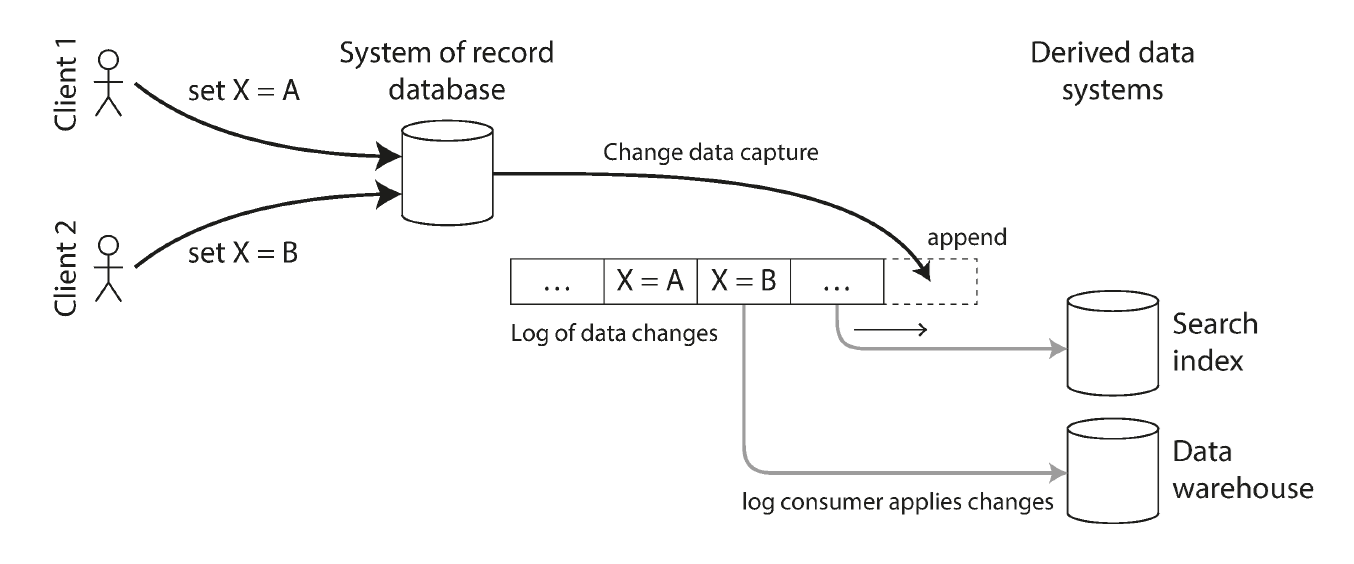
\includegraphics[width=0.8\textwidth]{resources/chapter-2/cdc.png}
    \caption{Ilustrasi CDC \parencite{dataIntensiveApplications}}
    \label{fig:cdc-illustration}
\end{figure}

PostgreSQL juga mendukung CDC dengan istilah \textit{logical replication}. Mekanisme ini menggunakan model \textit{publish} dan \textit{subscribe}. PostgreSQL yang mengirimkan log bertindak sebagai \textit{publisher}, lalu terdapat \textit{subscriber} lain yang mengonsumsi log yang dipublikasikan. \textit{Subscriber} ini bisa berupa replika PostgreSQL lagi atau aplikasi lainnya \parencite{pgLogicalReplication}.

PostgreSQL mendukung dua mode operasi untuk replikasi, yaitu replikasi secara asinkron dan sinkron \parencite{insideLogicalReplication}. Pada mode sinkron, \textit{subscriber} harus merespons terlebih dahulu terhadap perubahan data sebelum PostgreSQL dapat melakukan \textit{commit}.

\begin{figure}[htbp]
    \centering
    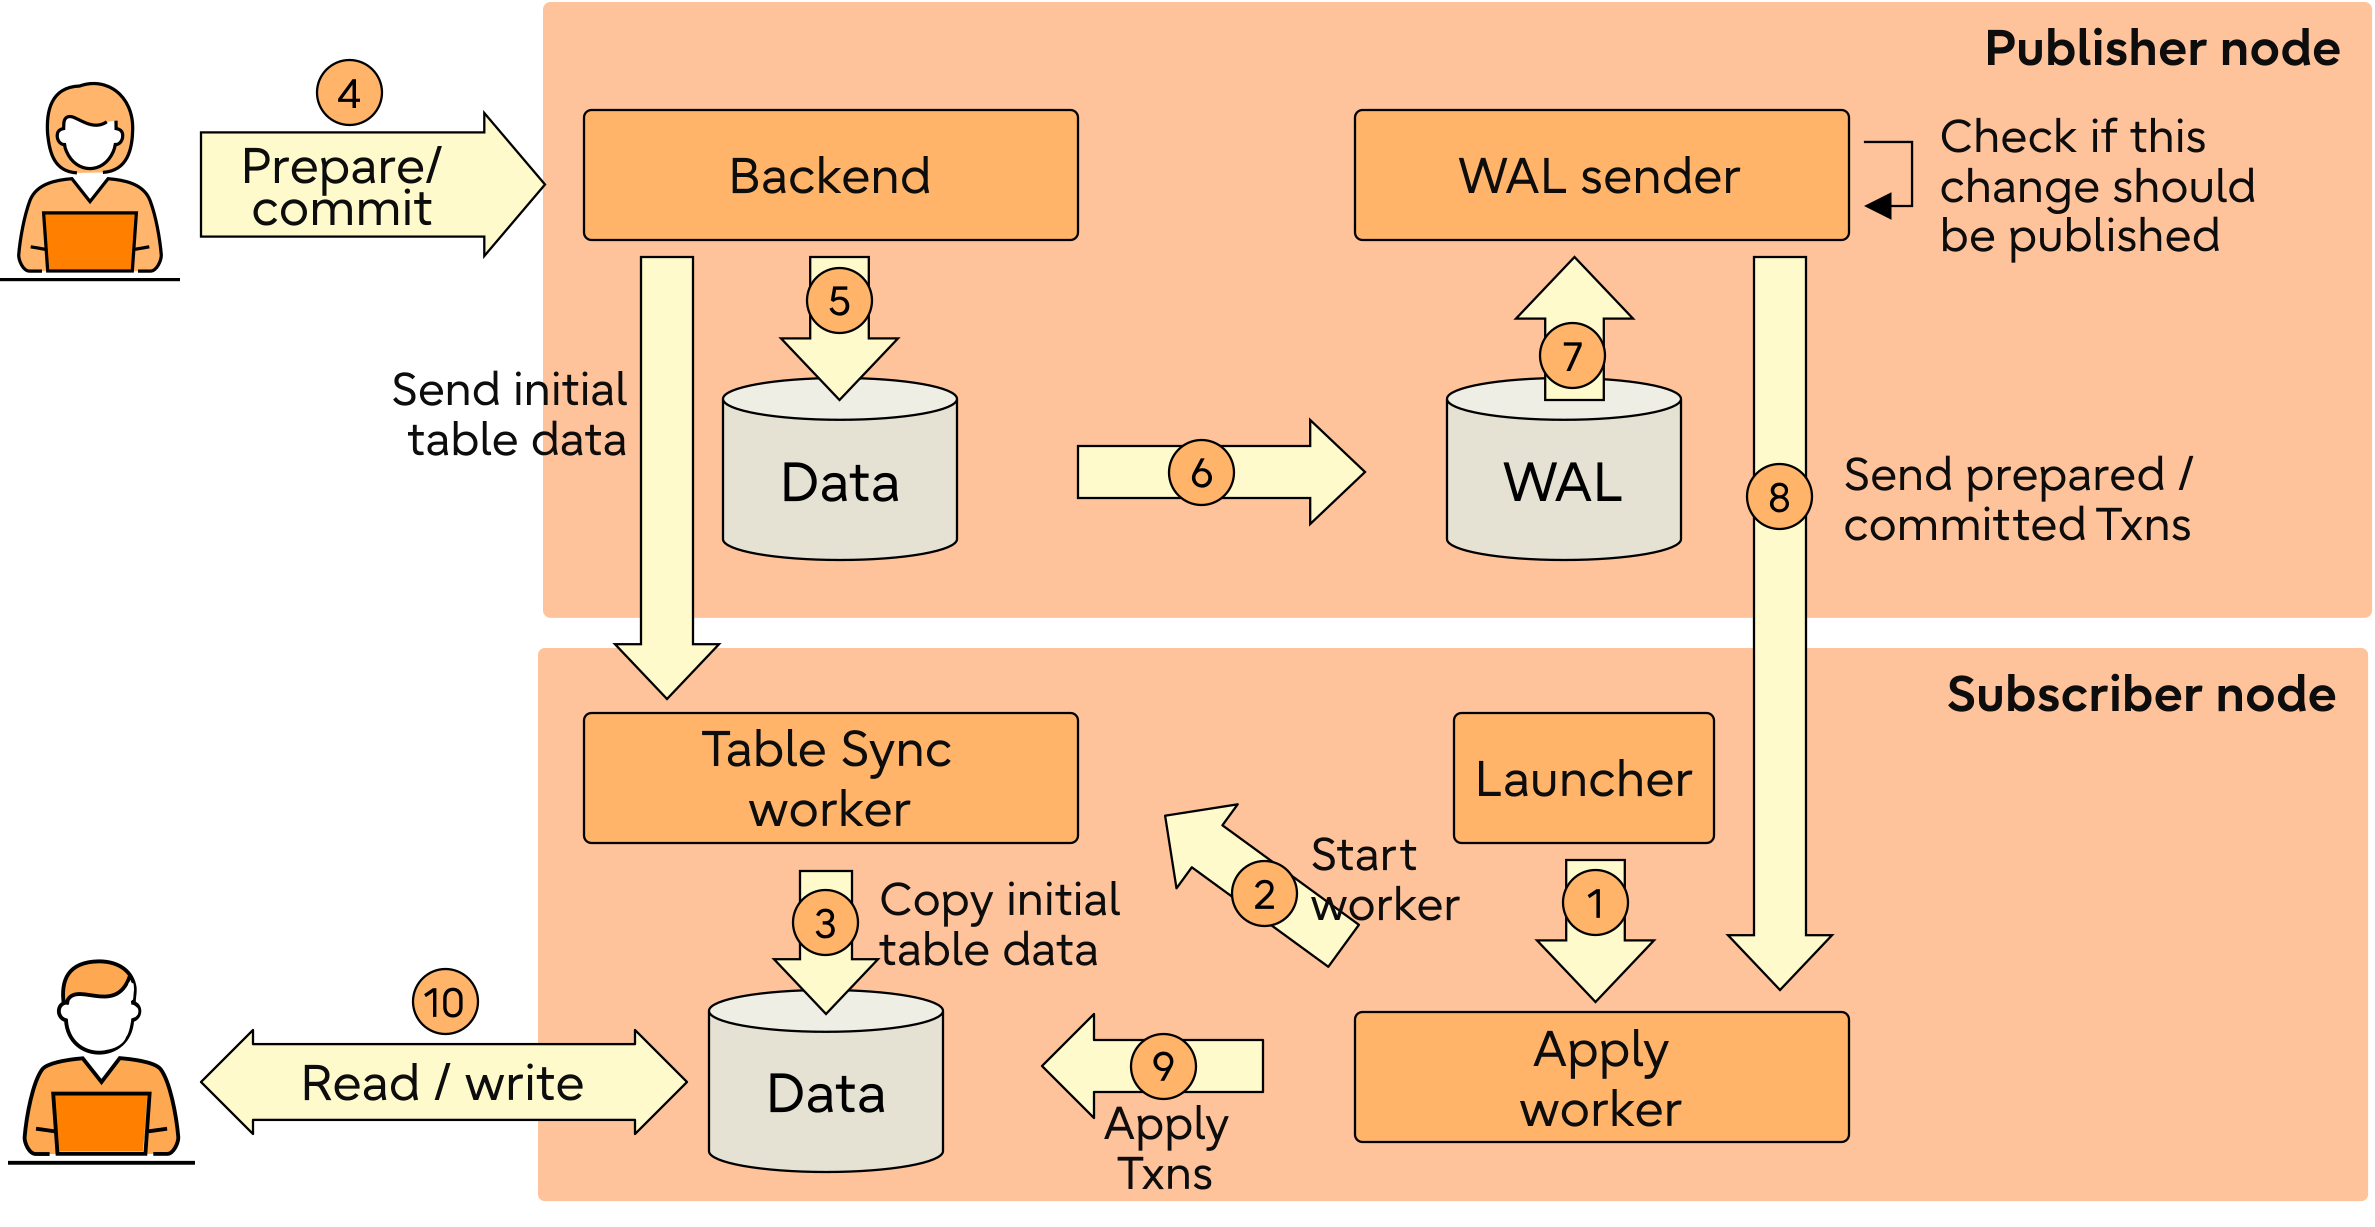
\includegraphics[width=0.8\textwidth]{resources/chapter-2/postgres-logical-replication.png}
    \caption{Arsitektur \textit{logical replication} \parencite{insideLogicalReplication}}
    \label{fig:logical-replication-architecture}
\end{figure}

